\documentclass{book}
\usepackage[utf8]{inputenc}
\usepackage{amssymb}
\usepackage{blindtext}
\usepackage[english]{babel}
\usepackage{graphicx}
\usepackage{wrapfig}
\usepackage[english]{babel}
\usepackage{algorithm}
\usepackage{algpseudocode}
\usepackage{amsthm}
\newtheorem{definition}{Definition}[section]
\newcommand{\norm}[1]{\left\lVert#1\right\rVert}
\newtheorem{theorem}{Theorem}[section]
\newtheorem{corollary}{Corollary}[theorem]
\newtheorem*{Importante}{\textbf{Importante}}
\newtheorem{lemma}[theorem]{Lemma}
\theoremstyle{definition}
\newtheorem{esempio}{\emph{Esempio}}
\usepackage{amsmath}
\usepackage{tikz}
\usetikzlibrary{shapes.geometric, arrows}
\usepackage{geometry}
\geometry{a4paper, top=2cm, bottom=2cm, left=1.5cm, right=1.5cm}
\usepackage{imakeidx}
\usepackage[T1]{fontenc}
\makeindex[columns=3, title=Alphabetical Index, intoc]
\title{Computer and Network Security}
\author{Lorenzo Rossi}
\graphicspath{{Images/}}
\begin{document}
\theoremstyle{definition}
\maketitle
\tableofcontents
\part{Third Midterm}
\chapter{Secret Sharing}
\section{Trivial Secret Sharing}\mbox{}\\
Supponiamo di avere un segreto e vogliamo dividerne la conoscenza in due persone (dette shareholders)\@.
Inoltre, vogliamo si viene a conoscenza del segreto se e solo se entrambe le parti rivelano la loro porzione di segreto.
\begin{figure*}[h]
    \centering
    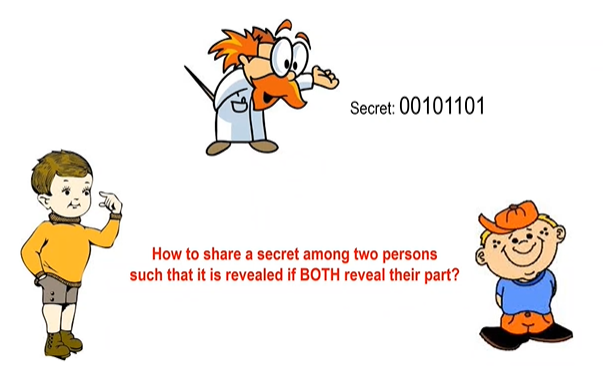
\includegraphics[scale=0.5]{2021-12-26-17-16-35.png}% chktex 8
\end{figure*}
Chi fornisce il segreto viene detto \textbf{dealer}, mentre chi riceve le porzioni del segreto sono detti \textbf{share}\@.\newline
Nel caso in cui avessimo diviso il segreto in parti uguali, è una pessima idea poiché per indovinare il segreto abbiamo \(\frac{1}{2^{N_{bit}}}\) probabilità di indovinare la password ed ora, avendo diviso il segreto in parti uguali, abbiamo una probabilità molto maggiore \(\frac{1}{2^{\frac{N_{bit}}{2}}}\) \@.
\subsection{XOR Secret Sharing}
Possiamo fare di meglio:\begin{enumerate}
    \item Prendi il segreto i.e.0010.1101;
    \item Genera una sequenza casuale \textbf{key} i.e.1011.0100;
    \item XOR il segreto e il valore casuale \textbf{one time pad} i.e.1001.1001;\newline
          Fino ad ora abbiamo applicato un \emph{Vernam cipher}\@.
    \item Diamo ad uno share la sequenza casuale, mentre ad un altro diamo il valore dello XOR;\@
    \item L'unione fra gli share da la chiave\@.
\end{enumerate}
\begin{Importante}
    Il conoscere la chiave, cioè il valore casuale, non mi da alcuna informazione riguardante la chiave\@.\newline Lo stesso discorso vale per il valore dello XOR poiché, come dimostrato nel \textbf{perfect secrecy}, l'operatore di XOR tra una stringa pseudocasuale e un valore casuale non da informazioni su quale sia la password\@.\newline
    Questi due aspetti rappresentano un requisito di sicurezza\@.
\end{Importante}
\newpage
\subsection{Modular Secret Sharing}
Un altro possibile schema è quello di utilizzare le somme modulari:\begin{enumerate}
    \item Prendi il segreto S in bit, trasformalo in digit i.e.0010.1101\(rightarrow\)45;
    \item Genera \(RAND\mod{N}\) i.e.\(RAND\mod{256} \rightarrow  180\);
    \item Esegui \(S-RAND\mod{N}\) i.e. \(S-RAND\mod{256}\rightarrow  121\);
\end{enumerate}
\begin{Importante}
    Questo schema è equivalente ad One Time Pad poiché abbiamo sommato un numero pseudocasuale con un numero casuare (in modulo)\@. In altre parole, la probabilità di indovinare S conoscendo il valore casuale o il valore della somma è uguale alla probabilità di indovinare senza sapere nulla\@.
\end{Importante}
Questo metodo è più facile da implementare per essere condiviso con N shareholders\@. In particolare, genero 3 quantità truly random ed effettua la differenza tra il segreto e queste 3 quantità modulo N\@.
Nel caso un attacker, riuscisse ad ottenere un numero sufficiente di share non può comunque ottenere la password, ma al più la differenza tra il segreto e le shares non prese\@.\newline Da qui è possibile definire il concetto di \textbf{perfect secrecy}: un avversario, conoscendo n-1 shares deve ancora possedere la probabilità di indovinare il segreto pari a quella di indovinare il segreto da zero\@.
\subsection{Shamir Secret Sharing}
Fino ad ora abbiamo costruito uno schema detto (n,n) secret sharing scheme in cui il primo parametro è il numero delle persone necessarie a rilevare il segreto e il secondo parametor è il numero di parti:\@il segreto viene rilevato solo se tutte le n parti forniscono il segreto\@.\newline
Un altro schema è \textbf(t,n) secret sharing scheme:\@il segreto è rilevato quando qualsiasi t delle n parti fornisce il segreto\@. Questo secondo problema è molto più complicato del trivial secret sharing\@.
\subsubsection{Idea:\@Schema (2,n)}
Il problema è quello di modellare uno schema per cui, conoscendo 2 degli n shareholders, posso ricostruire il segreto\@. Questo problema è riconducibile a quello di conoscere quanti punti sono necessari per definire una linea:\@ovviamente 2\@.
\begin{figure*}[h]
    \centering
    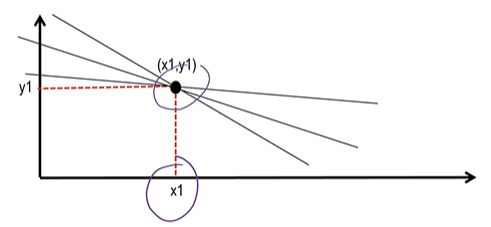
\includegraphics[scale=0.5]{2021-12-26-18-33-00.png}% chktex 8
\end{figure*}
Infatti conoscendo un solo punto (shares) ho infinite rette passanti per quel punto e quindi è impossibile ricondurci al segreto;\@tuttavia, conoscendo 2 punti (shares), tra essi passa solamente una sola retta e conseguentemente posso conoscere il segreto\@. Abbiamo comunque mantenuto la proprietà di poter avere un numero maggiore di 2 per ottenere il segreto, ma al minimo sono 2\@.
\subsubsection{Procedura: Schema\((2,n)\)}
\begin{itemize}
    \item \textbf{Dealer:} costruisce la linea:
          \begin{enumerate}
              \item Coefficiente a:\@scelto casualemnte;
              \item Segreto S:\@noto;
                    \begin{equation*}
                        \centering
                        y=S+ax
                    \end{equation*}
          \end{enumerate}
          Per esempio: \(a=15\quad S=39\)
    \item Distribuisci le shares ai n partecipanti scegliendo casualmente il valore \(x_{i}\) da introdurre nell'equazione della retta:
          \begin{itemize}
              \item Shareholder 1: \(x_{1}=1\rightarrow share=(1,54)\);
              \item Shareholder 2: \(x_{2}=2\rightarrow share=(2,69)\);
              \item Shareholder 3: \(x_{3}=3\rightarrow share=(3,84)\);
              \item \dots
          \end{itemize}
\end{itemize}
\begin{Importante}
    La y viene calcolata in base alla funzione della retta;\@tuttavia, i punti degli shareholder sono mantenuti con (x,y) e il valore delle \(x_{i}\) possono essere noti a priori a patto che la y sia nascosta\@.
\end{Importante}
\subsubsection{Procedura: Ricostruzione (2,n)}
\begin{itemize}
    \item Ricezione di due shares:\(P_{i}=(x_{i},y_{i})\quad P_{j}=(x_{j},y_{j})\);
    \item Interpola i punti per ricostruire l'equazione della retta:
          \begin{equation*}
              \centering
              \frac{y-y_{i}}{y_{i}-y_{j}}=\frac{x-x_{i}}{x_{i}-x_{j}}
          \end{equation*}
          Ottenendo:
          \begin{equation*}
              \centering
              y=y_{i}+\frac{x-x_{i}}{x_{i}-x_{j}}(y_{i}-y_{j})
          \end{equation*}
    \item Bisogna sostituire \(x=0\) per ottenere il segreto \(y=S\);
\end{itemize}
\subsubsection{Estensione al caso \((t,n)\)}
Estendendo il discorso precedentemente introdotto, ci si riconduce al caso di polinomi di grado \(t-1\) unicamente definiti da \(t\) punti:
\begin{itemize}
    \item Linea:\@2 punti;
    \item Parabola (quadratic):\@3 punti;
    \item Cubiche:\@4 punti;
    \item \dots
\end{itemize}
\subsubsection{Generalizzazione: Schema \((t,n)\)}
\begin{itemize}
    \item \textbf{Dealer}:\
          \begin{enumerate}
              \item Genera un polinomio casuale \(p(x)\) di grado \(t-1\);
              \item Imposta il segreto \(s\) come il termine noto del polinomio:
                    \begin{equation*}
                        p(x)=s+a_{1}x+a_{2}x^{2}+ \cdots +a_{t-2}x^{t-2}+a_{t-1}x^t-1
                    \end{equation*}
                    con s il segreto e i coefficienti delle x generati truly random;
              \item Distribuisci uno share ad ogni shareholders:
                    \begin{equation*}
                        \centering
                        (x_{i},y_{i})\rightarrow y_{i}=p(x_{i})
                    \end{equation*}
          \end{enumerate}
    \item \textbf{Ricostruzione}: Colleziona \(t\) shares su \(n\) disponibili e calcola il segreto utilizzando \emph{l'Interporlazione di Lagrange} con \(x=0\):
          \begin{equation*}
              \centering
              s=\sum_{shares\ x_i}{y_{i}\Lambda_{x_{i}}}\quad with\quad\Lambda_{x_{i}}=\Lambda_{x_{i}}(0)=\prod_{shares\ x_{k}\neq x_{j}}{\frac{-x_{k}}{x_{i}-x_{k}}}
          \end{equation*}
          L'interpolazione di Lagrange si basa sul concetto che qualsiasi polinomio di grando t-1 con t punti noti, può essere decomposto come:
          \begin{equation*}
              \centering
              y=\sum_{i=1}^{t}{y_{i}\Lambda_{i}(x)}
          \end{equation*}
          In cui \(\Lambda_{i}(x)\) è la base del polinomio calcolata come:
          \begin{equation*}
              \centering
              \Lambda_{i}(x)=\prod_{m=1,m\neq1}^{l}{\frac{x-x_{m}}{x_{i}-x_{m}}}\quad \Lambda_{i}(x_{i})=1;\quad \Lambda_{i}(x_{m})=0\quad for\ m\neq i
          \end{equation*}
\end{itemize}
\subsubsection{Segretezza}
Per discutere di quanto sia sicuro questo schema dobbiamo ricordare che in questo ambito la segretezza è così definita:
\begin{center}
    \emph{Finché si conoscono (t-1) shares non si dovrebbe avere nessuna informazione sul segreto che stiamo condividendo.}
\end{center}
Lo schema di Shamir in questo senso non è sicuro poiché se conoscessi a priori il range in cui è compreso il segreto, potrei ciclare su uno share mancante per ottenere un segreto nel range voluto\@.
\begin{esempio}
    Effttuiamo uno schema (3,4) in cui per conoscere il segreto dobbiamo conoscore almeno 3 share su 4\@. Dato che utilizziamo l'interpolazione di Lagrange il polinomio sarà di grado \(t-1\) e il termine noto sarà \(s\):
    \begin{equation*}
        y=3 x^2+52 x+32;
    \end{equation*}
    Abbiamo 4 shareholders, quindi dobbiamo generare 4 punti,generando un valore casuale x e sostituendolo nell'equazione precedente. Avendo posto rispettivamte i valori \(1,2,3,4\), si ottengono i seguenit punti:
    \begin{equation*}
        (1,87),(2,148),(3,215),(4,288)
    \end{equation*}
    Ora, occorre calcolare i valori di lambda, supponendo di aver collezionato \(x_{1},x_{2},x_{3}\), come
    \begin{equation*}
        \centering
        \Lambda_{i}(x)=\prod_{m=1,m\neq1}^{l}{\frac{x-x_{m}}{x_{i}-x_{m}}}\quad \Lambda_{i}(x_{i})=1;\quad \Lambda_{i}(x_{m})=0\quad for\ m\neq i
    \end{equation*}
    Ottenendo:
    \begin{equation*}
        \Lambda_{1}(x)=\frac{(x-\text{x2}) (x-\text{x3}) }{(\text{x1}-\text{x2}) (\text{x1}-\text{x3}) }
    \end{equation*}
    \begin{equation*}
        \Lambda_{2}(x)=\frac{(x-\text{x1}) (x-\text{x3}) }{(\text{x2}-\text{x1}) (\text{x2}-\text{x3}) }
    \end{equation*}
    \begin{equation*}
        \Lambda_{3}(x)= \frac{(x-\text{x1}) (x-\text{x2}) }{(\text{x3}-\text{x1}) (\text{x3}-\text{x2}) }
    \end{equation*}
    Ora, per ricostruire il segreto occorre applicare
    \begin{equation*}
        \centering
        y=\sum_{i=1}^{t}{y_{i}\Lambda_{i}(x)}
    \end{equation*}
    Quindi:
    \begin{equation*}
        s=y_{1}\Lambda_{x_{1}}(0)+y_{2}\Lambda_{x_{2}}(0)+y_{3}\Lambda_{x_{3}}(0)=87(30)+148(-3)+215(1)=32
    \end{equation*}
    Ora supponiamo di non sapere uno share \emph(\(d\)) e vogliamo verificare se questo schema garantisce secrecy o meno\@. Sostituendo imponiamo:
    \begin{equation*}
        s=y_{1}\Lambda_{x_{1}}(0)+d\Lambda_{x_{2}}(0)+y_{3}\Lambda_{x_{3}}(0)= 476-3d
    \end{equation*}
    Ipotizziamo che il range in cui vive s è noto e compreso tra 0 e 100\@. Possiamo indovinare il segreto? Si, basta ciclare sulle d:\begin{itemize}
        \item Con \(d=125\rightarrow s=101\);
        \item Con \(d=126\rightarrow s=98\);
        \item Con \(d=127\rightarrow s=95\);
        \item Da varie prove si capisce che d è nel range \(126\leq d\leq 158\);
    \end{itemize}
    Quindi, conoscere 2 su 3 in uno schema 3 su 4 ci permette di escludere tutti i valori d non ammissibili\@.
\end{esempio}
\subsubsection{Real Shamir Secret Sharing}
Lo schema reale utilizza l'aritmetica modulare (con \(p\) numero primo) invece di quella reale e  le operazioni effettuate sia con il segreto sia con il polinomio devono essere scelti nel campo dei numeri primi\@.\newline
L'interpolazione rimane uguale\@.
\begin{Importante}
    La regola per scegliere il numero primo p deve essere più grande del dominio del segreto per avere un segreto uniformemente distribuito e non è necessario che sia grande\@.
\end{Importante}
\end{document}